\section{Previo}

\noindent \justifying


\subsection{¿Qué métodos se pueden utilizar para resolver ecuaciones en diferencias en el dominio del tiempo discreto?} 

\begin{itemize}
	\item Convolción discreta.
	\item Transformada discreta de Fourier
	\item Transformada discreta de Laplace
	\item Transformada Z
\end{itemize} 


\subsection{¿Cuál es la relación entre las variables s y z? ¿Cómo se relaciona el plano complejo en s con el plano complejo en z?}


\subsubsection{Transformada Z}

\begin{itemize}
	\item Es una una nueva herramienta matemática que simplifica el análisis y la síntesis de los sistemas discretos lineales e invariantes en el tiempo.
	\item Análoga: \begin{itemize}
		\item  transformada de Laplace que se emplea en el estudio de los sistemas continuos lineales
		e invariantes en el tiempo.
		\item la transformada z se utiliza en el análisis de los sistemas discretos lineales e invariantes en el tiempo.
	\end{itemize}
	\item Permite realizar operaciones, “ver” propiedades y características de
	las señales y los sistemas discretos en una forma más simple que en el dominio del tiempo
\end{itemize}

Vamos a discretizar una señal pasando de la figura (a) a la (c) de la figura \ref{fig:000002}, y con ella haremos movimientos hasta llegar a (a) .



\begin{figure}[H]
	\centering
	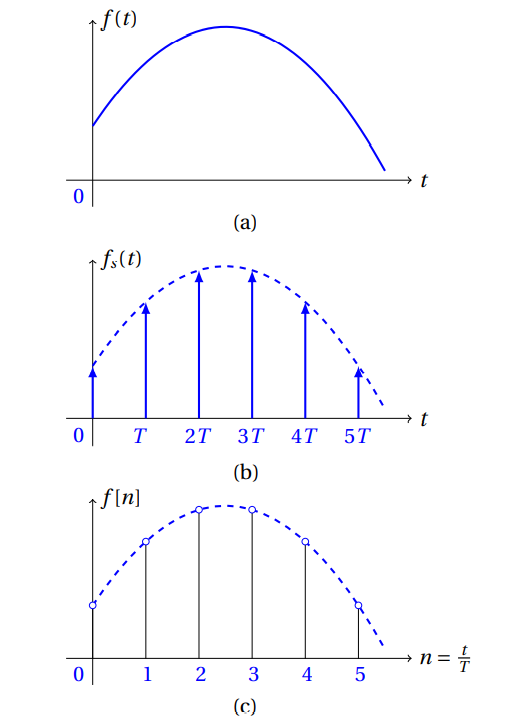
\includegraphics[scale=0.5]{000002}
	\caption{(a) Señal continua. (b) Señal muestreada. (c) Señal discreta.}
	\label{fig:000002}
\end{figure}

\setlength{\abovedisplayshortskip}{10pt}
%\setlength{\belowdisplayshortskip}{10pt}
%\setlength{\belowdisplayskip}{0pt}
\addtolength{\jot}{0.5em}

\begin{align}
	f_{S}(t) &=f(t) \delta_{T}(t)=f(t) \sum_{n=0}^{\infty} \delta(t-n T)=\sum_{n=0}^{\infty} f[n T] \delta(t-n T) \\
	F_{s}(s) &=\mathscr{L}\left\{f_{s}(t)\right\}=\sum_{n=0}^{\infty} f[n T] e^{-n T s} \label{cu-2} \\ 
	z & =e^{s T}=e^{(\sigma+j \omega) T}=e^{\sigma T} e^{j \omega T} \\
	F(z) &=\left.\mathscr{L}\left\{f_{s}(t)\right\}\right|_{z=e^{s T}}=\mathcal{Z}\{f[nT]\}=\sum_{n=0}^{\infty} f[n T] z^{-n} \label{cu4}
\end{align}

\begin{itemize}
	\item Podemos decir que la transformada de Laplace unilateral es la ecuación \ref{cu4}.
	\item \textbf{Región de convergenica:}
	\begin{itemize}
		\item Usualmente se abrevia como ROC.
		\item Es conjunto de valores $z$ que verifican la convergencia $F(z)$.
	\end{itemize}
\end{itemize}

\subsubsection{Mapeo}
\begin{itemize}
	\item se puede considerar un mapeo del plano complejo s al plano complejo z visto en la ecuación \ref{cu-2}.
	\item Dominio: 
	$$ z=e^{s T}=e^{\sigma T} e^{j \omega T}=e^{\sigma T} e^{j(\omega T+2 \pi k)}$$
	\subitem Cuando se recorre el eje imaginario desde $ - \infty$ a $ + \infty$, el círculo unitario se delinea un número infinito de veces.
\end{itemize}

Se tiene que saber que recordar los mapeos de ecuaciones vistos en Matemáticas Avanzadas, son de alguna manera muy útiles. Uno de los casos más frecuentes es es cuando $\sigma <0$ , $ |z|=e^{\sigma T}<1$ el semiplano izquierdo del plano s se mapea en el interior del círculo unitario
del plano z. Se puede apreciar ello en la figura \ref{fig:000004}. Recuerda eso es para dar una idea pero existen múltiples configuraciones e intersecciones que se tienen que profundizar.


\begin{figure}[H]
	\centering
	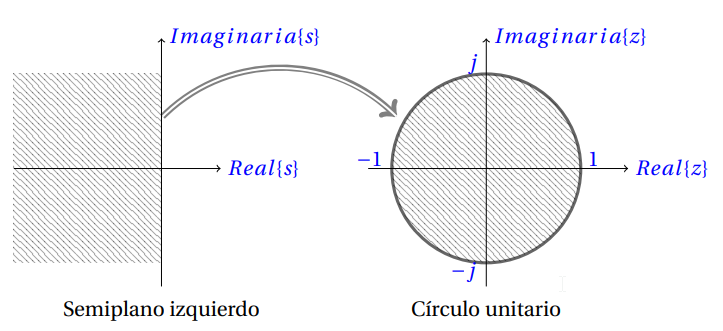
\includegraphics[scale=0.5]{000004}
	\caption{Mapeo del plano s al plano z, con $z=e^{sT}$.}
	\label{fig:000004}
\end{figure}

\subsection{¿Cómo se caracteriza la estabilidad de los sistemas lineales e invariantes de tiempo discreto?}

	
	Un sistema discreto es BIBO si para cada entrada de $x[n]$ está acotada, de forma que si existe una $M<\infty$ que cumpla con que $|x[n]|>M$ para tona n, y cada salida de $y[n]$ está igualmente acotada.
	
	\begin{equation}
	|x[n]| \leq M < \infty
	\end{equation}
	
	La anterior ecuación nos indica que va a existir un valor M que va a acotar a todos los valores x[n] de la señal de entrada.
	
	En cambio, un sistema de tiempo discreto LTI es BIBO estable si y solo si su secuencia de respuesta de impulso {h [n]} es absolutamente sumable, es decir,
	\begin{equation}
		S=\sum_{n=-\infty}^{\infty}|h[n]|<\infty
	\end{equation}
	
	\noindent\textbf{Demostración:}

	Partimos de lo siguiente
	\begin{equation}
		|x[n]| \leq M_x < \infty
	\end{equation}		
	
	Empecemos considerando a la salida de la señal como una función convolución
	\begin{equation}
		y[n]=x[n]*h[n]=\sum_{m=-\infty}^{\infty}x[m]h[n-m]
	\end{equation}
	
	Si aplicamos valor absoluto a ambos lados de la ecuación y usamos la desigualdad de tres componentes en la suma obtenemos: 
	\begin{equation}
		\lvert y[n]\rvert = \lvert \sum_{m=-\infty}^{\infty}x[m]h[n-m] \rvert \leq \sum_{m=-\infty}^{\infty}x[m]h[n-m]
	\end{equation}		
	\begin{equation}
		=\sum_{m=-\infty}^{\infty}\lvert x[m]h[n-m] \rvert \leq \sum_{m=-\infty}^{\infty}M_x \lvert h[n-m] \rvert
	\end{equation}
	\begin{equation}
		\leq M_x \sum_{m=-\infty}^{\infty} \lvert h[n-m] \rvert = M_xS
	\end{equation}

	Si $S<\infty$ tenemos que 
	
	\begin{equation}
		|y[n]|\leq B_y < \infty
	\end{equation}
	
	Para demostrar la convergencia de S consideramos la entrada x[n] de la siguiente forma
	
	\[
	x[n]=
	\begin{cases}
		$sgn(h[-n])$, & \text{si h[-n]  $\neq$ 0} \\
		K, & \text{si h[-n] = 0}				\end{cases}
	\]
	
	Donde sgn(c)=1 si $c>0$ y sgn(c)=-1 si $c<0$ y $|K| \leq 1$
	\newline
	
	Si usamos la entrada n=0 tenemos:
	\begin{equation}
		y[0]=\sum_{k=-\infty}^\infty sng(h[k]) h[k] = S \leq B_y < \infty
	\end{equation}
	Con lo que se demuestra que $|y[n]| \leq B_Y$ que implica que $S\leq\infty$

\subsection{¿Qué diferencias existen entre los métodos de fracciones parciales para sistemas de tiempo continuo y sistemas de tiempo discreto?}

Ambos métodos son usados para obtener la anti transformada de Laplace y Z respectivamente. En el caso de sistemas de tiempo discreto el método es mejor conocido como expansión de fracciones parciales, y difiere con el método de sistemas continuos en los siguientes aspectos:\\
1. Cada fracción va multiplicada por un factor z que facilita su anti transformación.\\
2. Se considera un primer coeficiente que no va acompañado de ningún factor calculado de las siguiente forma:

%$$d_{0}=\frac{b_{m}}{(−p_{1})(−p_{2})...(−p_{n})}$$

\begin{equation}
	d_{0}=\frac{b_{m}}{(- p_{1})(- p_{2}) \cdots (- p_{n})}
\end{equation}

Donde m=número de ceros y n= número de polos.\\    
El método de fracciones parciales para sistemas de tiempo discreto es idéntico al que se utiliza en la transformada de Laplace (tiempo continuo), y requiere que todos los términos de la expansión en fracciones parciales se puedan reconocer fácilmente en la tabla de pares de transformadas Z.\\
Si X(z) tiene uno o más ceros en el origen (z = 0), entonces X(z)/z ó X(z) se expande en la suma de términos sencillos de primer o segundo orden mediante la expansión en fracciones parciales, y se emplea una tabla de transformadas Z para encontrar la función del tiempo correspondiente para cada uno de los términos expandidos.\\    
Del mismo modo que en sistemas de tiempo continuo y teniendo en cuenta la fracción:\\
\[
F(z)=\frac{N(z)}{D(z)}=\frac{N(z)}{(Z+P_{1})(Z+P_{2})(Z+P_{3})...(Z+P_{i})}
\]
Donde P1, P2, P3 ... Pi son las raíces del polinomio, estas raíces podrán ser: reales simples, reales múltiples, complejas simples, complejas múltiples.

\subsection{¿En qué dispositivo de la vida cotidiana se realizan conversiones de señales de tiempo continuo a tiempo discreto y viceversa?}

	
	\textbf{Convertidor DAC (Digital a Análoga)}
	\begin{itemize}
		\item La salida digital de una computadora puede convertirse en una señal de control analógica para ajustar la velocidad de un motor o para controlar alguna variable física.
		\item Las computadoras pueden ser programados para generar señales analógicas necesarias para analizar circuitos analógicos
		\item Para ser escuchado sonido de los altavoces utilizan DAC para convertir una señal digital, guardada en un CD o un reproductor mp3) en una señal a analógica. Esos DAC son usados por los lectores de CD, reproductores digitales de música y tarjetas de sonido.
	\end{itemize}
	
	\textbf{Convertidor ACD (Análoga a Digital}
	\begin{itemize}
		\item Son usados en cualquier dispositivo que tenga sensores de temperatura.
		\item En los automóviles con sensores de proximidad.
		\item Dispositivos de almacenamiento y procesamiento de audio.
	\end{itemize}
	

%\section{Preguntas de cierre}

%\subsection{Explique brevemente la importancia de la conversión de señales de tiempo continuo a tiempo discreto}
%\subsection{¿Qué relación existe entre la transformadas de Laplace y Z?}
%\subsection{¿Cómo se caracteriza la estabilidad de sistemas de tiempo continuo y tiempo discreto en el contexto de funciones de transferencia?}